\subsection{On the mehcanism of modes $A'$ and $QS$}

\begin{figure}
  \centering
  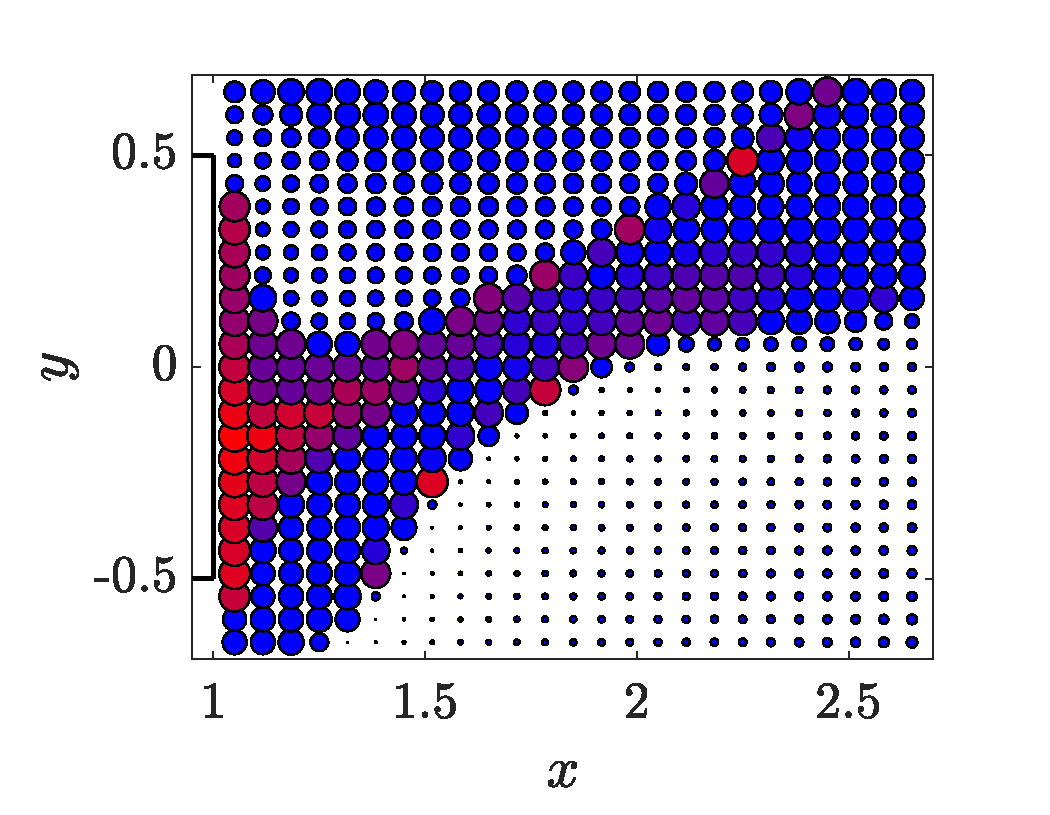
\includegraphics[width=0.49\textwidth]{./fig/LagTrac/part_AR1_Re200.eps}
  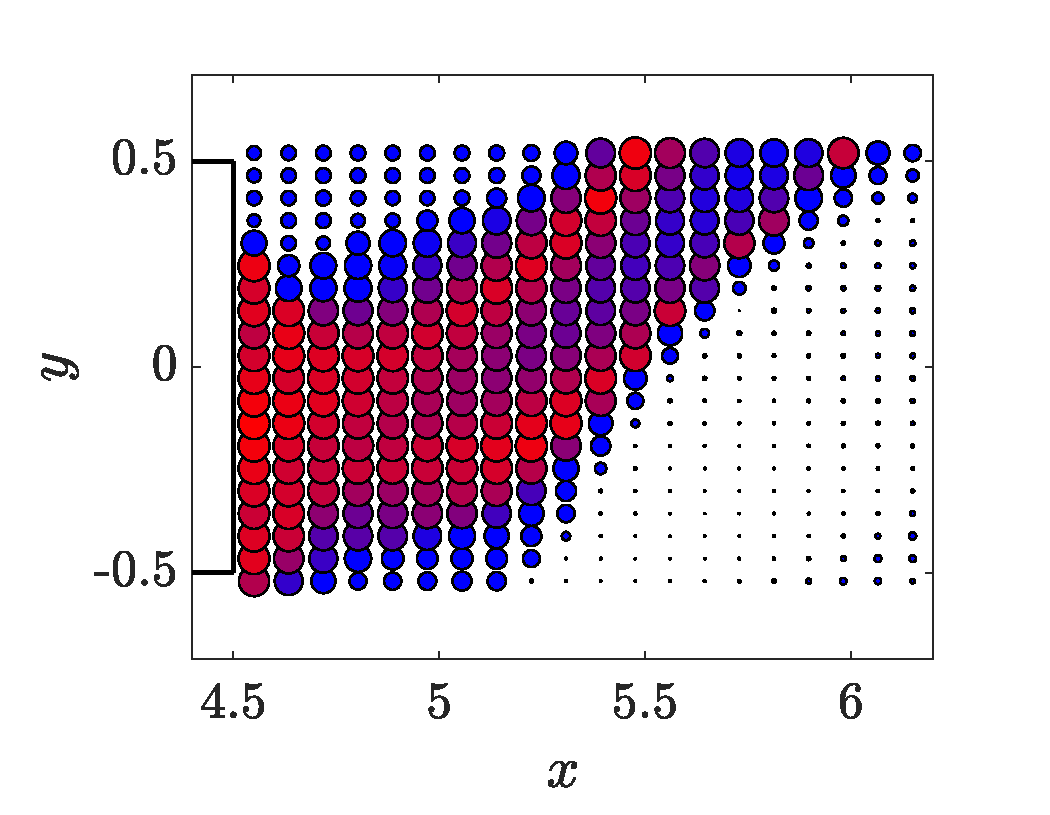
\includegraphics[width=0.49\textwidth]{./fig/LagTrac/part_AR4p5_Re410.eps}
  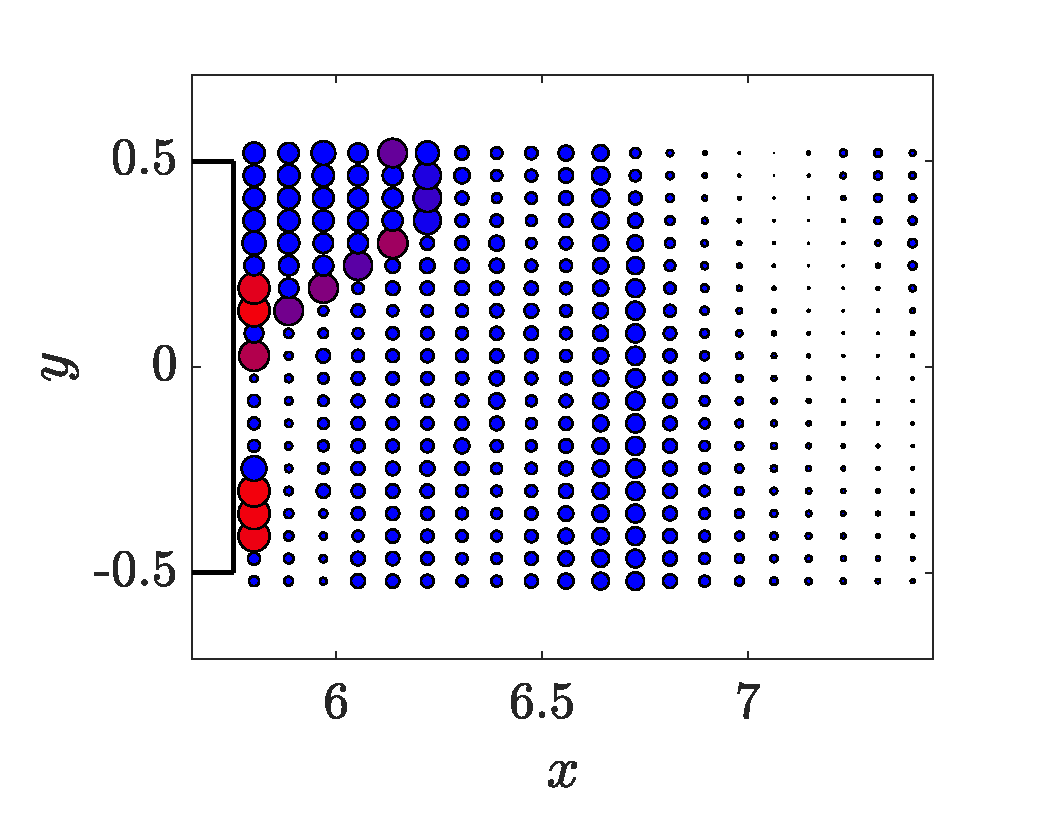
\includegraphics[width=0.49\textwidth]{./fig/LagTrac/part_AR5p75_Re550.eps}
  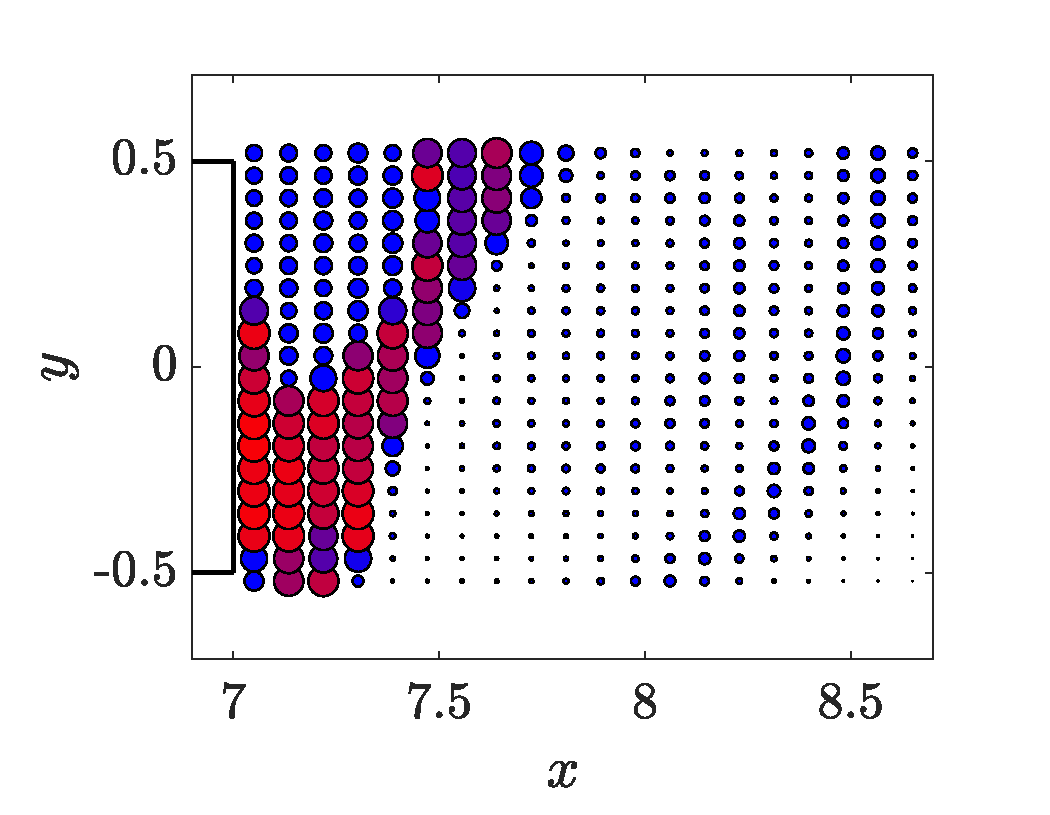
\includegraphics[width=0.49\textwidth]{./fig/LagTrac/part_AR7_Re500.eps}  
  \caption{XX AUMENTARE IL RANGE INVESTIGATO XX}
  \label{fig:part_res}
\end{figure}    

\begin{figure}
  \centering
  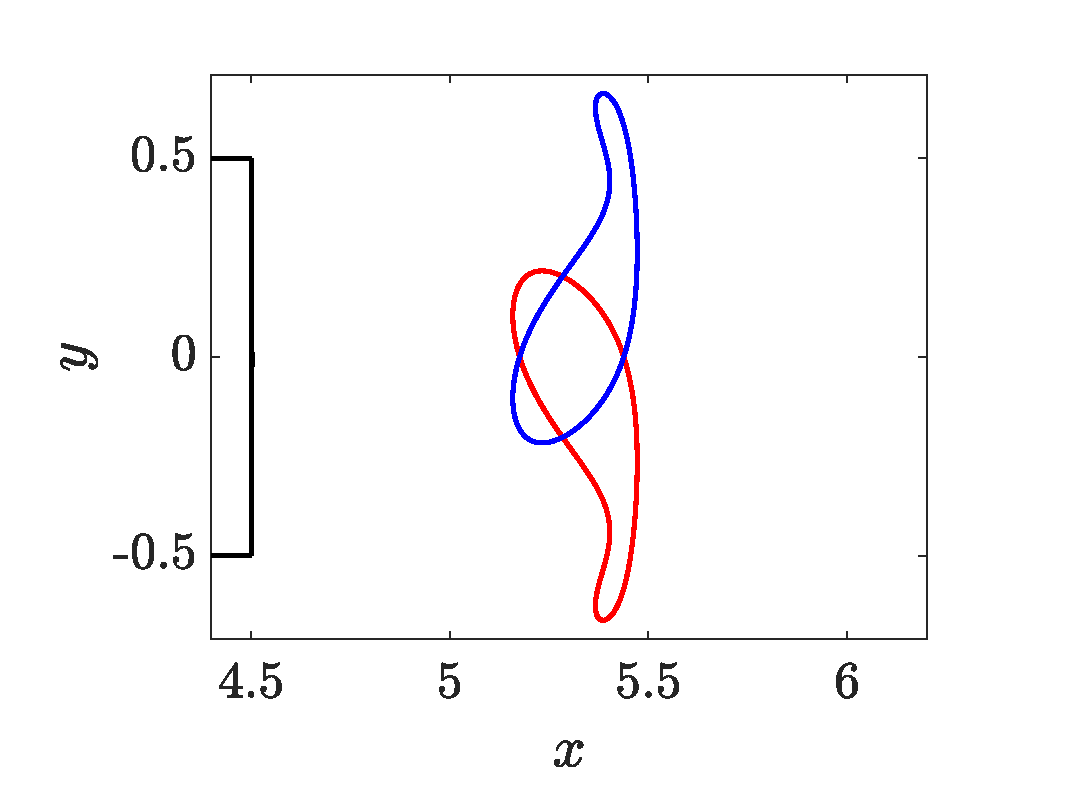
\includegraphics[width=0.49\textwidth]{./fig/LagTrac/orb_AR4p5_Re410.eps}   
  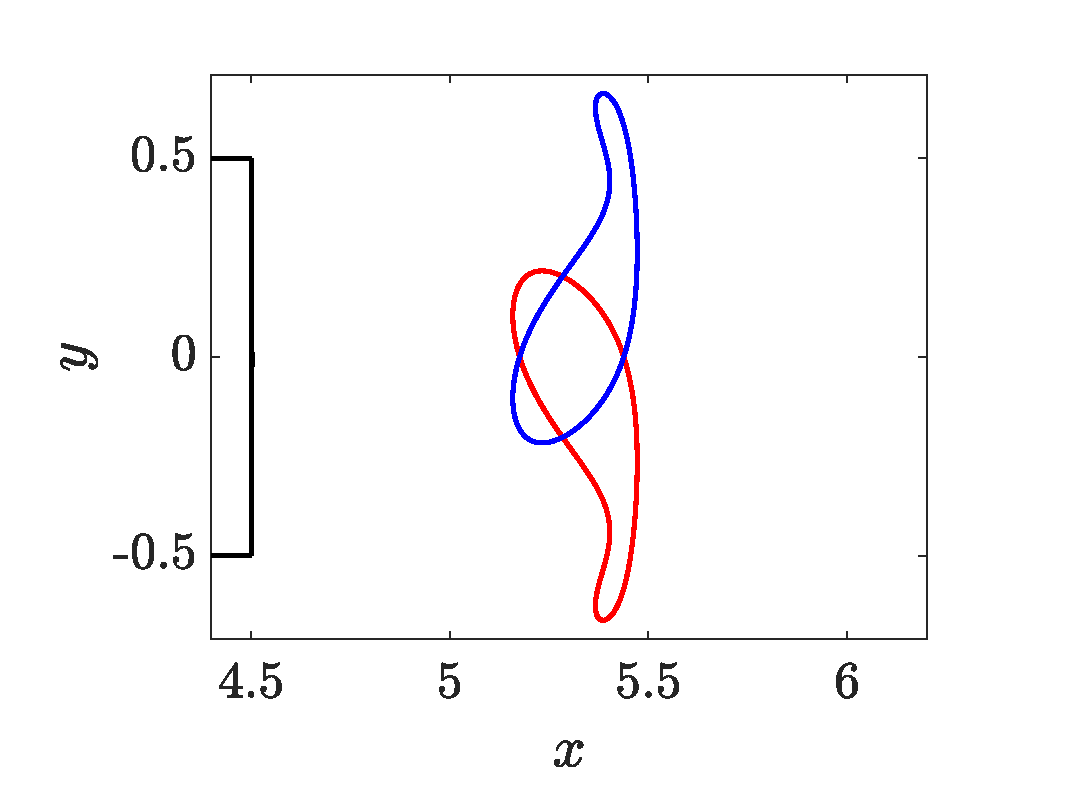
\includegraphics[width=0.49\textwidth]{./fig/LagTrac/orb_AR4p5_Re410.eps} 
  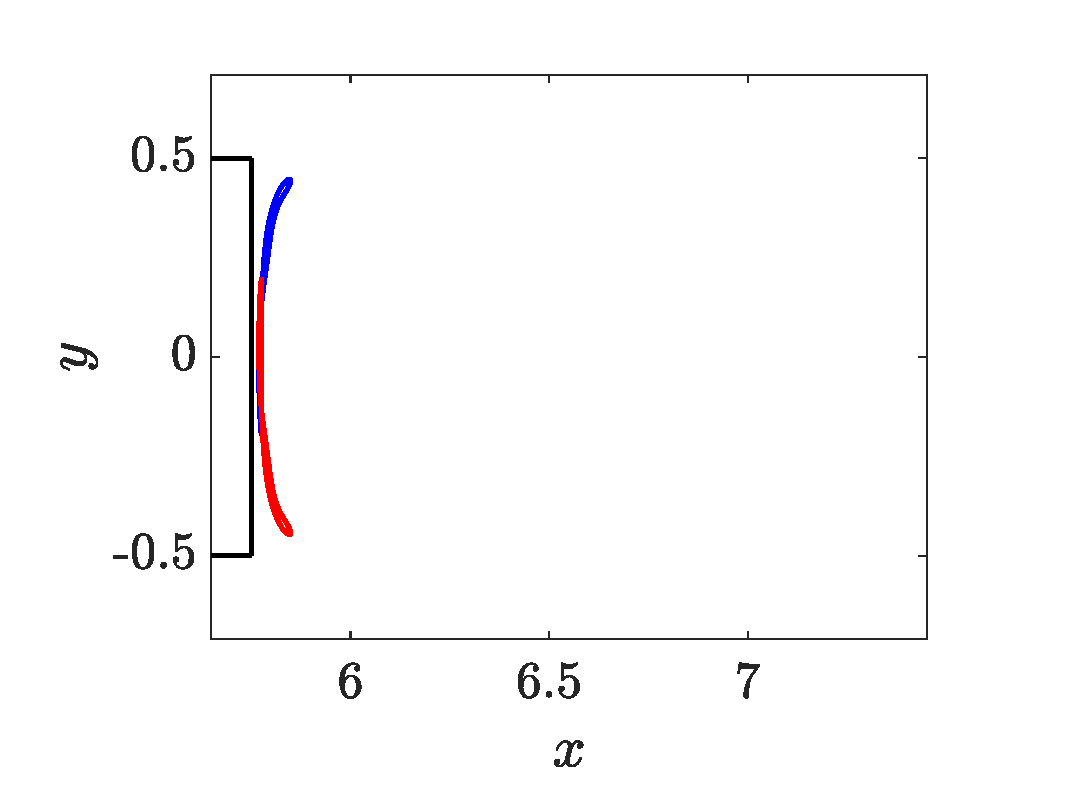
\includegraphics[width=0.49\textwidth]{./fig/LagTrac/orb_AR5p75_Re550.eps}
  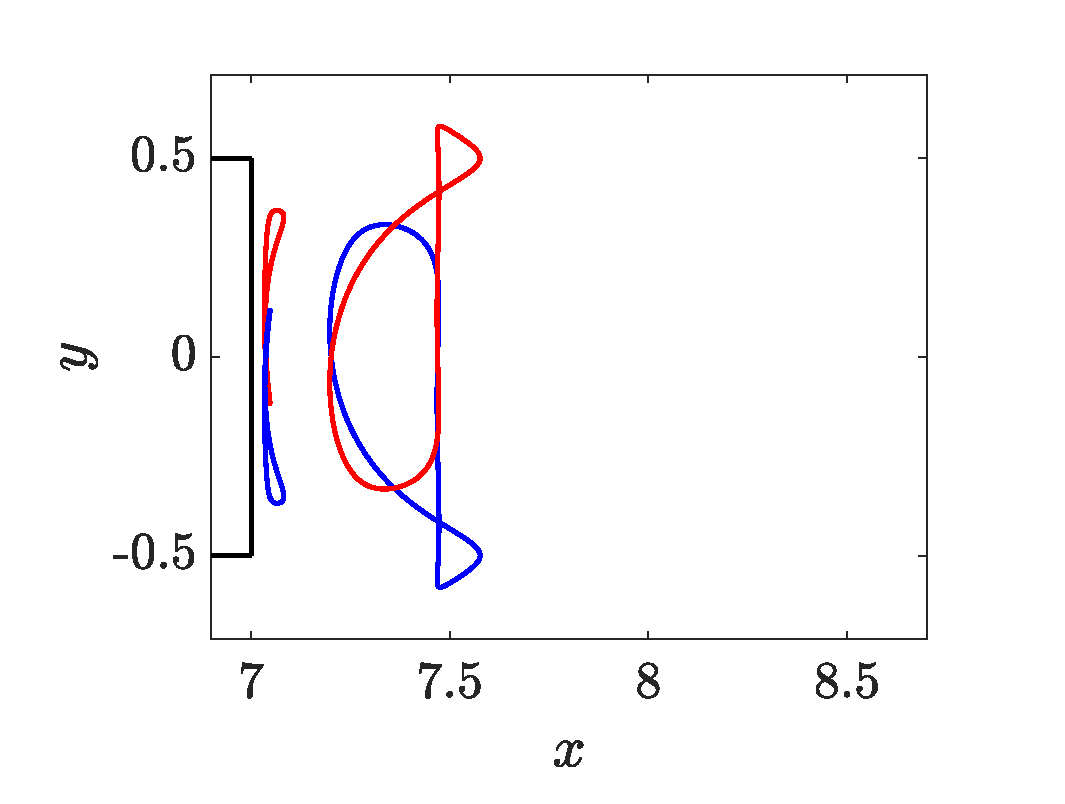
\includegraphics[width=0.49\textwidth]{./fig/LagTrac/orb_AR7_Re500.eps}
  \caption{XX AUMENTARE IL RANGE INVESTIGATO XX}
  \label{fig:part_res}
\end{figure}

\begin{figure}
  \centering
  \includegraphics[width=0.49\textwidth]{./fig/AR5s/Ener_AR5p5_Re450_Re550_beta2.png}
  \includegraphics[width=0.49\textwidth]{./fig/AR5s/Prod_AR5p5_Re450_Re550_beta2.png}
  \includegraphics[width=0.49\textwidth]{./fig/AR5s/Trsp_AR5p5_Re450_Re550_beta2.png}
  \includegraphics[width=0.49\textwidth]{./fig/AR5s/Diss_AR5p5_Re450_Re550_beta2.png}
  \caption{Budget of energy for mode $A'$ (top) and mode $QS$ (bottom). $\AR=5.5$ and $Re=450$ (for mode $A'$) and $Re=550$ (for mode $QS$). Top left: $u_i u_i^*$. Top right: Production. Bottom left: Transport. Bottom right: Dissipation.}
  \label{fig:budget_ener}
\end{figure}
